\chapter{Learning from Monolingual Data}
\label{chap:monolingual}
While in this work our target languages are under-resourced, we have many
resources available for the source languages. We would like to use these to
make better sense of the input text, giving our classifiers clearer signals and
better representations for lexical selection in the target language. The
approaches considered in this chapter make additional features or different
representations available to the CL-WSD classifiers based on knowledge of the
source language, either gleaned through unsupervised methods or baked into
extant tools. Since we have relatively little bitext available for
Spanish-Guaraní and Spanish-Quechua, we will need to lean more on our Spanish
resources, software and data, in order to make better sense of the input text.

Perhaps most saliently for Spanish, we have abundant monolingual text
available, which suggests that we could use unsupervised methods to discover
regularities in the language, yielding better features for our classifiers.
This approach has been broadly successful in the literature
\cite{turian-ratinov-bengio:2010:ACL,baroni2014don}, and here we adapt some of
the methods explored in previous work on text classification to our task.

Concretely, in this chapter we explore labels learned from existing NLP tools
such as off-the-shelf taggers and parsers for Spanish, Brown clustering
\cite{brown1992class}, and a few related approaches to neural embeddings. There
are of course other related methods that one could investigate, especially
making use of the broader literature on distributional semantics, but these
will be left to future work. First we will describe the methods used in some
detail, and then towards the end of the chapter, in Section
\ref{sec:monolingual-experiments}, we describe experiments and present
experimental results.

\section{Monolingual features from other NLP tools}
There are a large number off-the-shelf NLP tools available for Spanish. Here we
will look into part of speech taggers and syntactic parsers specifically.
Tagging can help us capture abstractions over particular word types, and
provides some disambiguation on its own. For example, in Spanish, \emph{poder}
can be the infinitive verb ``to be able", or it can be a noun, meaning ``power,
ability". And if these different meanings are surfaced as different words in
the target language (as they are in English), then simply having an accurate
POS tag makes the CL-WSD task much easier. More generally, perhaps a noun in
the window surrounding a focus word could be indicative of a particular
meaning.

Similarly, syntactic structure may also provide useful features.  Verbs
especially may have drastically different translations in the target language
based on their objects. There are many familiar examples of this phenomenon,
especially among the ``light verbs" and ``phrasal verbs" with noncompositional
meanings in English and Spanish.

In the Chipa software, we can make use of arbitrary annotations for the input
text (see Section \ref{sec:annotations}), so adding more features based on
analysis by external tools is straightforward.

As a first step, we synthesize features based on the part-of-speech tags of the
tokens in a window around the current focus word, and using a syntactic parser,
the heads and children of the current focus word. In principle, we could use
other annotations, such as sense annotations from a monolingual WSD system,
given a good one. This idea is akin to one that we will explore in Chapter
\ref{chap:multilingual}, in which we use Chipa itself (trained for other
language pairs, and with larger data sets) to provide annotations, effectively
using some other target language as a tagset for WSD.

For POS tagging, we run the open source FreeLing text analysis suite
\cite{padro12} on input sentences. FreeLing can perform a number of analyses
for Spanish, including POS tagging, dependency parsing, lemmatization, and
named entity recognition, of which the latter two are part of the standard
preprocessing done for all experiments in this work. When all the text for an
experiment is known beforehand, as in the experiments reported in this chapter,
we can run FreeLing during the data annotation step (see Section
\ref{sec:datasetsandpreprocessing}) and simply record FreeLing's output as text
annotations. When running on novel test sentences, as in server mode, we must
run it on those sentences just before inference time.

Similarly, for syntactic features, we use MaltParser\cite{Nivre06maltparser:a}
\footnote{Available at \url{http://maltparser.org/} ; in this work we use
version 1.9.0 of the parser, and the ``espmalt" pretrained model, which is
available at \url{http://www.iula.upf.edu/recurs01_mpars_uk.htm}, and was
trained on the IULA Treebank\cite{MARIMON12.519}, by researchers from the IULA
group at Universitat Pompeu Fabra.} to get dependency parses of the input
sentence. This is also performed as a corpus annotation, making the syntactic
relationships for each token available during feature extraction. The parser
here depends on the POS tags produced by FreeLing. Conveniently, FreeLing and
the espmalt parser model assume the same tag set, but as with any pipeline of
NLP systems, using the inferred output from the tagger as input to the parser
carries the risk that errors at early stages in the pipeline could propagate
and cause problems at the later stages of processing. Here we note this concern
but move on; it is a very general problem, and solutions to it are an open area
of research. The parser also depends on the coarse-grained ``universal" POS
tags \cite{PETROV12.274}, which we manually map from the IULA tagset to
universal coarse tags during corpus annotation.

Operationally, before training our CL-WSD system, we parse all of the training
data with the ``espmalt" model, using the tags inferred by FreeLing during
preprocessing. The dependency parses output by MaltParser are stored on disk in
CONLL-X format. Then with a corpus annotation script, we walk the dependency
graphs to find each token's immediate syntactic head (or the root of the
sentence) and every token's immediate syntactic children, if any. All of these
dependency heads and children are annotated in the training data, to be made
available during feature extraction. Then at feature extraction time, chipa
turns these stored annotations into sparse binary features. The list of all
syntactic features made available to the classifier is given in Figure
\ref{fig:syntacticfeatures}.

\begin{figure*}
  \begin{centering}
  \begin{tabular}{|r|p{11cm}|}
    \hline
    name          & description  \\
    \hline
    \texttt{postag}    & part-of-speech tag for the focus token \\
    \hline
    \texttt{postag\_left}  & POS tag for the token to the left of focus token \\
    \hline
    \texttt{postag\_right} & \emph{ibid.}, for the right \\
    \hline
    \texttt{head\_lemma} & lemma of the focus word's syntactic head, or ROOT if
    it has no head). \\
    \hline
    \texttt{head\_surface} & \emph{ibid.}, but for the syntactic head's surface
    form. \\
    \hline
    \texttt{child\_lemma} & lemma of the syntactic child or children of the
    focus word. Feature appears multiple times for multiple children. \\
    \hline
    \texttt{child\_surface} & \emph{ibid.}, but for the children's surface
    forms. \\
    \hline
  \end{tabular}
  \end{centering}
  \caption{Additional syntactic features}
  \label{fig:syntacticfeatures}
\end{figure*}

\section{Brown Clustering}
The Brown clustering algorithm\cite{brown1992class}, also known as IBM
clustering, as it was developed by the Candide group at IBM, takes an
unannotated text corpus as input and assigns each word type found the corpus
into hierarchical clusters, such that types in the same cluster have similar
usage patterns based on the bigram statistics of the corpus. The tree of
clusters is binary-branching, so the identity of a cluster is simply its path
from the root of the tree, and clusters that are close in the tree have similar
usage patterns. The desired number of ``leaf" clusters must be set ahead of
time as a tunable parameter.

Each of the word types present in the input corpus is allocated to one of the
leaf clusters, such that the assignment attempts to maximize the probability of
the input corpus.  These clusters were originally intended for use in
class-based language modeling, and as such the scoring function is the mutual
information between subsequent tokens. Concretely, the optimization process is
searching for a clustering $C$ that maximizes the probability of the corpus
$\boldsymbol{w}$, according to the formula in Figure \ref{fig:brownprob}.

\begin{figure*}

  \begin{equation} \label{eq:brownclassprob}
  P(\boldsymbol{w}; C) = \prod_{w_i} p(w_i | C(w_i)) p(C(w_i) | C(w_{i-1}))
  \end{equation}

  \caption{The Brown clustering expression for the probability of a corpus with
  a specific clustering $C$. It is the product, for each token, of the
  probability of that token given its cluster, and the probability of that
  current cluster given the previous cluster. This is analogous to the
  ``emission" and ``transition" probabilities used in an HMM-based tagger.}
  \label{fig:brownprob}
\end{figure*}

Finding an optimal assignment of all word types in the corpus into these
hierarchical clusters is an intractable problem, but several greedy approaches
that find local optima have been explored in the literature.  Notably, in
addition to Liang's approach, Franz Och's \texttt{mkcls} package (familiar to
Moses users, and described in \cite{och1999efficient}) optimizes the same
function when assigning words to classes. In any case, with the available
software running on modern hardware, we can find a clustering for the corpora
used in this work in a fairly short time, on the order of hours.

Here our immediate use for these clusters is to create more features for our
classifiers, interpreting the clusters into which a word type falls as a tag
for instances of that type. These annotations give a more abstract, less sparse
representation than surface forms or lemmas, hopefully providing useful
semantic and syntactic generalizations. We may also preprocess the input to
the clustering algorithm beforehand, as long as we can reproduce the
preprocessing for unseen input text at query time.

In applying Brown clusters to this task, we would like to answer several
questions.

\begin{itemize}
  \item Can learning Brown clusters from monolingual source text improve our
  performance on this CL-WSD task?
  \item Does more source-language text help us learn more helpful Brown
  clusters, with respect to the CL-WSD task? Can a large enough monolingual
  corpus help us overcome domain mismatches?
  \item What kinds of preprocessing should we do on the source text?
  Particularly, should Spanish source text be lemmatized?
\end{itemize}

\subsection{Clustering in practice}
In this work we use Percy Liang's implementation \footnote{Available at
\url{https://github.com/percyliang/brown-cluster}} of Brown clustering
\cite{Liang05semi-supervisedlearning}. We ran this tool on two different
monolingual corpora, the Spanish section of the Europarl corpus \cite{europarl}
(2 million sentences) and a dump of Spanish-language Wikipedia (20 million
sentences). In all cases, we set the number of leaf clusters to 1000, which is
the default for the package.
When working with Spanish, considering its relative morphological richness, we
may consider lemmatizing our input text before clustering. This decision will
be more significant than it would be for English, given the inflections present
in Spanish, especially verb conjugations and adjective-noun agreement.
We might expect that Brown clustering on surface forms would help us find
abstractions over syntax, but perhaps lemmatization will turn it toward more
semantic abstractions. This is an empirical question, and we briefly look into
it here, first by qualitatively examining the clusters that we learned, but
later extrinsically evaluating the clusters to see how they affect the CL-WSD
task.

\begin{figure*}[t!]
  \begin{tabular}{|r|p{10cm}|}
    \hline
    category  & top twenty word types by frequency \\
    \hline
    countries &  \\
    \hline
    more places & \\
    \hline
    mostly people & \\
    \hline
    infrastructure & \\
    \hline
    common verbs & \\
    \hline
  \end{tabular}
\caption{Selected clusters found in the surface version of Spanish Europarl}
\label{fig:clusters-europarl-surface}
\end{figure*}

\begin{figure*}[t!]
  \begin{tabular}{|r|p{10cm}|}
    \hline
    cluster description  & top twenty word types by frequency \\
    \hline
    countries & francia irlanda alemania grecia italia españa rumanía portugal polonia suecia bulgaria austria finlandia hungría bélgica japón gran\_bretaña dinamarca luxemburgo bosnia \\
    \hline
    more places & kosovo internet bruselas áfrica iraq lisboa chipre afganistán estrasburgo oriente\_próximo copenhague asia chechenia gaza oriente\_medio birmania londres irlanda\_del\_norte berlín barcelona \\
    \hline
    mostly people & hombre periodista jefes\_de\_estado individuo profesor soldado abogado delincuente demócrata dictador iglesia alumno adolescente perro chico economista gato jurista caballero bebé \\
    \hline
    infrastructure & infraestructura vehículo buque servicio\_público cultivo edificio barco negocio motor avión monopolio planta ruta coche libro aparato tren billete actividad\_económica camión \\
    \hline
    common verbs & pagar comprar vender explotar practicar soportar exportar comer consumir suministrar sacrificar fabricar gobernar comercializar cultivar fumar capturar almacenar curar beber \\
    \hline
  \end{tabular}
\caption{Selected clusters found in the lemmatized version of Spanish Europarl}
\label{fig:clusters-europarl-lemma}
\end{figure*}

\begin{figure*}[t!]
  \begin{tabular}{|r|p{10cm}|}
    \hline
    category  & top twenty word types by frequency \\
    \hline
    countries &  \\
    \hline
    more places & \\
    \hline
    mostly people & \\
    \hline
    infrastructure & \\
    \hline
    common verbs & \\
    \hline
  \end{tabular}
\caption{Selected clusters found in the surface version of Spanish Wikipedia}
\label{fig:clusters-wikipedia-surface}
\end{figure*}

\begin{figure*}[t!]
  \begin{tabular}{|r|p{10cm}|}
    \hline
    category  & top twenty word types by frequency \\
    \hline
    countries &  \\
    \hline
    more places & \\
    \hline
    mostly people & \\
    \hline
    infrastructure & \\
    \hline
    common verbs & \\
    \hline
  \end{tabular}
\caption{Selected clusters found in the lemmatized version of Spanish Wikipedia}
\label{fig:clusters-wikipedia-lemma}
\end{figure*}



Figures \ref{fig:clusters-europarl-surface}, \ref{fig:clusters-europarl-lemma},
\ref{fig:clusters-wikipedia-surface} and \ref{fig:clusters-wikipedia-lemma}
show some hand-selected illustrative examples of clusters that we found in our
monolingual Spanish corpora, Europarl and Wikipedia, in both surface-form and
lemmatized versions. Examining the output of the clustering algorithm, we see
some intuitively satisfying results; there are clusters corresponding to the
names of many countries, nouns referring to people by profession, and some
semantically similar verbs. The words listed in these figures are the top
twenty terms from that cluster, by frequency in the corpus. Note that the names
given for the clusters were also chosen by hand, rather than through some
automatic process. It is reassuring that the clustering process, over all of
these corpora, is finding some interpretable generalizations in the text.

Comparing the lemmatized versus the surface-form versions of the clustering, we
note that, as expected, the clusters capture more syntactic regularities when
given the inflected forms. Consider, for example the cluster containing
\emph{infraestructura} in Figure \ref{fig:clusters-europarl-lemma}, as compared
to its cluster in Figure \ref{fig:clusters-europarl-surface}. In the lemmatized
version, we see that \emph{infraestructura} falls into a cluster primarily
composed of words pertaining to transportation-related concepts, such as
\emph{vehículo} 'vehicle', \emph{billete} 'ticket' and \emph{avión} 'airplane'.
In the Wikipedia lemma clusters, shown in Figure
\ref{fig:clusters-wikipedia-lemma}, we see some satisfying semantic clusters as
well, such as adjectives describing political positions, verbs about making
choices, and a cluster of locations, mostly cities.

Contrastingly, on the surface-form side, the cluster that contains
\emph{infraestructura} does not immediately reveal the same conceptual
similarity: we see \emph{formación} 'education (formal)' \emph{creatividad}
'creativity', and \emph{comida} 'food' in the same cluster. While a few of the
words have similar meanings, the clustering seems to have found that these
words cluster together as singular feminine nouns, which is more of a
syntactic commonality than a semantic one. This is not to say that the
surface-form clusters do not exhibit semantic relatedness; in the ``profession
nouns" cluster in Figure \ref{fig:clusters-wikipedia-surface}, we see nouns
that refer to people's professions, although it should also be noted that these
are all singular masculine nouns. Also in the Wikipedia surface clusters, we
see a cluster containing almost entirely words referring to cardinal
directions\footnote{With the inclusion of \emph{voivodato} (English:
'voivodeship' or Polish 'województwo') which, I have just learned from
Wikipedia, is an administrative region in eastern Europe, similar to a
historical duchy or modern province.}.

So a qualitative look at the clusters found in these corpora shows some
promising regularities found in the text. As expected, when we cluster on the
surface forms, we find both syntactic and semantic similarities, but using the
lemmatized forms seems to push the clusters towards conceptual similarity. It
is still an empirical question which of these approaches will help more for our
CL-WSD task, but we will try them both.

\subsection{Classification features based on Brown clusters}
Given a clustering learned from a large monolingual corpus, we must still
decide how to extract classification features from those clusters. If we know,
for example, that the token to the left of the focus word is in cluster
``010111111100", what information do we provide to the classifier? We could
interpret this cluster atomically, as a tag for that token, and create sparse
features for an input sentence based on the clusters present in it, perhaps
focusing on the window surrounding the focus word. However, following the work
of Turian \emph{et al.} \cite{turian-ratinov-bengio:2010:ACL}, we also take the
prefixes of each cluster's bit strings at 4, 6, and 10 bits, taking advantage
of the hierarchical structure in the clusters, and used these separate sparse
features.

As a concrete example using the lemmatized Wikipedia clusters, if we find that
the lemma \emph{rioplatense} is in a three-token window around the current
focus word, and that this lemma in in cluster ``111110111111111110", then we
extract the following features, setting each of them to $1$.

\begin{itemize}
\item \texttt{brown\_window\_wikipedia\_lemma(111110111111111110)}
\item \texttt{brown\_window\_wikipedia\_lemma\_4(1111)}
\item \texttt{brown\_window\_wikipedia\_lemma\_6(111110)}
\item \texttt{brown\_window\_wikipedia\_lemma\_10(1111101111)}
\end{itemize}

We additionally extract analogous features for all tokens in the sentence;
these would be called \texttt{brown\_bag\_wikipedia\_lemma},
\texttt{brown\_bag\_wikipedia\_4}, and so on. If we are using clusters based on
the surface forms, these simply do not have \texttt{lemma} in their name, and
features based on Europarl, are marked with \texttt{europarl} rather than
\texttt{wikipedia}.

\begin{figure*}
  \begin{centering}
  \begin{tabular}{|r|p{11cm}|}
    \hline
    name          & description  \\
    \hline
    \texttt{brown\_bag}    & Bag of all Brown clusters for the entire sentence \\
    \hline
    \texttt{brown\_window}  & All Brown clusters for the three-token window around the focus word \\
    \hline
  \end{tabular}
  \end{centering}
  \caption{Features extracted from Brown clusters. These came in surface-form
  and lemma variants, and were trained on both the Europarl for Spanish, and
  our Wikipedia dump. Additionally, we add variants for the 4, 6, and 10-bit
  prefixes of the clusters.}
  \label{fig:brownfeatures}
\end{figure*}

In cases of unknown words, where we do not have a cluster assignment for a word
in the input text, we simply do not extract cluster features for that word.
This will happen in practice, even for a fairly large monolingual corpus, but
may be especially common in this setting due to domain mismatches. Many
biblical names, for example, are not present in Europarl.

\section{Neural Word Embeddings}
Another rich source of features that has proved useful for many text
classification problems in recent years is neural word embeddings, perhaps most
famously developed in the work of Mikolov et al. \cite{mikolovword2vec} and
their associated open source implementation of the technique,
word2vec\footnote{Available at
\url{https://code.google.com/archive/p/word2vec/}}. In this work we investigate
the use of ``word2vec"-style word embeddings, as well as the related technique,
``doc2vec" or ``paragraph vectors"
\cite{dai-document-embedding-2015,quocle-distributed-representations-2014}.
These techniques let our classifiers operate on lower-dimensional dense vectors
(of a few hundred dimensions, typically), as opposed to the high-dimensional
sparse vectors typically used in earlier NLP literature\footnote{
What we might consider to be ``symbolic" binary features used in machine
learning systems for NLP in recent decades -- such as ``the word `dog` appears
in the sentence" -- are effectively equivalent to these very sparse ``one hot"
representations of words, in which, for a vocabulary of size $|V|$, words are
represented by a length-$V$ vector in which all but one of the elements are 0}.

There is a rich literature on continuous representations for words; the idea
has a long lineage in NLP, and we could try any number of dimensionality
reduction or distributional semantics approaches here. However, recent
empirical work by Baroni et al \cite{baroni2014don} (summed up by the title of
the paper, ``Don't Count, Predict!") has shown that representations built
during discriminative learning tasks are typically more effective for text
classification problems similar to ours.

Unlike Brown Clustering, which infers hierarchical clusters for each word type,
but like other embedding techniques, word2vec learns multidimensional
representations for word types, turning the very sparse ``one hot"
representation in which words with similar uses or meanings do not have any
obvious similarity into a much denser continuous space, wherein words with
related meanings are placed nearby. These ``embeddings", or placements of word
types in a continuous space, are learned latently during some other
classification task, and are performed by the early layers of a neural network.

The word2vec model in particular has two variations, useful in different
contexts. One, called Continuous Bag-of-Words (CBOW) learns a classifier that
can predict individual words based on their context, while the ``skip-grams"
variant does the reverse and learns to predict context words based on an
individual focus word. The received wisdom\footnote{According to the TensorFlow
tutorial on word2vec, available at
\url{https://www.tensorflow.org/tutorials/word2vec}} is that CBOW is more
appropriate when training on smaller data sets, but this is an empirical
question and here we try out both variants.

In either case, running a word2vec training process results in a static mapping
from word types to their embeddings in a vector space of a given size,
typically a few hundred dimensions. These embeddings have been shown to be
helpful as features in a number of different NLP tasks \cite{baroni2014don},
allowing us to learn richer representations of word types from plentiful
unannotated monolingual text. This effectively turns what was a purely
supervised task, requiring labeled training data, into a semi-supervised task,
in which the representation-learning phase can be carried out on unlabeled data
by synthesizing a supervised learning task that can be performed with simple
monolingual text as its training data.

We trained a variety of word2vec embeddings for our text classification tasks,
again training on the Spanish-language section of the Europarl corpus (roughly
57 million words or 2 million sentences) and a dump of Spanish Wikipedia (449
million words, 20 million sentences). We learned embeddings using both CBOW and
skip-gram approaches, in 50, 100, 200, and 400 dimensions. In all cases, we
used the associated \texttt{word2phrase} tool, distributed with the public
\texttt{word2vec} implementation, which finds collocations in the input text
and treats them as individual tokens. The same collocations must be identified
in the input text for their embeddings to be used. At lookup time, we keep a
list of all the multiword expressions present in the dictionary of embeddings,
sorted from longest to shortest, first considering number of tokens, then
breaking ties by considering number of characters, and greedily replace any of
these multiword expressions (starting with the longest) found in the input text
with the token representing that MWE.

\subsection{From word embeddings to classification features}
We should note that, like Brown clusters, the embeddings learned for a word
type are fixed for that word type, and do not reflect the context of a
particular token, so a focus word's embedding vector will not provide useful
classification features on its own. This leaves us with the problem of how to
make use of the word vectors in a given sentence. Concretely, we must decide
how to combine several word vectors together, and which word vectors in a
sentence to choose for combination. A typical approach is to take element-wise
sums or averages over the embedding vectors for the tokens in a context
\cite[Chapter 8]{Goldberg17}.

There are a variety of approaches we could take, even within summing and
averaging. We could sum (element-wise) all of the word vectors for all the
tokens in the entire sentence. We could only consider the words in a narrow
window around the focus word. Or we could perform a weighted sum, in which
words nearer to the focus word are given more weight, but these weights drop
off according to some function, scaling with the distance from the focus word.
For our experiments here, we try these three different approaches, resulting in
three different feature sets.

In the first feature set, called ``window", we present the classifier with the
element-wise sum of the vectors for the focus word (or the token containing the
focus word, if it is inside a multi-word expression) and the three tokens on
either side. The resulting vector thus has the same dimensionality as the word
embeddings that we learned. Secondly, in the ``fullsent" feature set, we
perform an unweighted element-wise sum of the word embeddings for the entire
input sentence. Finally, in the ``pyramid" feature set, we sum the embeddings
for each token in a broad window around the focus word, but before summing,
scale each embeddings by $max(0, 1.0 - (0.1 * d))$, where $d$ is the distance
between that token and the focus word.

For all of the variations considered here, whether we are using skipgrams or
CBOW, for whichever dimensionality we choose, and for any of the methods of
combining the vectors, when using these word embeddings without other
resources, we end up representing a CL-WSD problem as a sentence a dense vector
of the same dimensionality as the word embeddings that we are currently using,
and these dense vectors can be passed along to any machine learning algorithm
that we care to use.

\section{Neural Document Embeddings}
Rather than coming up with representations for individual words and then
combining them to get a representation of a sentence or a local context, we
might want a technique that directly finds representations of sequences of
text. One such technique, called ``paragraph vectors" or ``doc2vec", does just
this. doc2vec was developed by some of the same researchers that produced
word2vec, and it can build representations for arbitrary sequences of text,
rather than individual word types
\cite{dai-document-embedding-2015,quocle-distributed-representations-2014}.
This approach takes unlabeled text and learns representations for word types
jointly with representations for each \emph{document}. Here a ``document" is an
arbitrary sequence of tokens, perhaps a single sentence, or perhaps much
longer, depending on the intended application.

Similar to word2vec, here doc2vec uses a neural network with a single hidden
layer to predict words in the current context. Here however, the hidden layer
contains not only an embedding trained for word types, but also an embedding
for the current document. Training proceeds by loading the current
representation for the current word and the current document, attempting to
predict some other word in the context (analogous to training for word2vec),
and then updating both of these representations based on the gradients between
the desired output and the actual output. 

Also similar to word2vec, there are two variants of the approach that can be
used for training. One variant of doc2vec, the ``Distributed Memory Model of
Paragraph Vectors", uses a paragraph embedding combined with word embeddings
for several words in the current context to predict a single individual word.
The other variant, the ``Distributed Bag of Words model of Paragraph Vectors",
simply uses the current paragraph vector to predict all of the words in the
current context, which despite containing ``bag of words" in its name, is more
closely analogous to the skip-gram artitecture for word2vec
\cite{quocle-distributed-representations-2014}, since the model is trained to
predict the entire context based on a single embedding.

In either case, the resulting stored model consists of the embeddings for
individual word types. The embeddings for any particular document in the
training set are not stored, since that document is unlikely to appear again at
inference time, but the embeddings for individual word types provide a useful
generalization, since they constrain embeddings for new documents.

At inference time, doc2vec produces new vectors representing previously unseen
documents based on these fixed word embedding vectors. In our work, as in many
text classification tasks, documents will be input sentences, or perhaps
sentence-length Bible verses, or smaller windows of text around a
word-in-context. To produce a representation for a new document, the embeddings
for word types are held constant and we run stochastic gradient descent
optimization to infer an embedding for the current document, based on the fixed
word embeddings, such that it helps predict words in the current context.

doc2vec thus provides a straightforward approach for learning to produce
representations of new documents, based on an unlabeled training corpus. Here
we use the implementation of doc2vec provided by the gensim package
\cite{rehurek-lrec} \footnote{Available at
\url{https://radimrehurek.com/gensim/}}, with its default settings, which uses
the ``distributed memory" model.

During training data annotation, we pass over our bitext corpus, take the
source-language sentence from each training pair, and infer a new embedding for
it based on a doc2vec model trained on our 20 million sentences from
Spanish-language Wikipedia. These sentence-level embeddings are stored as a
token annotation on the first token of each sentence, so they can be made
available during feature extraction. We can also show the gensim software a
small context window around the focus word, rather than the entire sentence to
generate a more focused representation.

In either case, the result is a dense vector of the specified dimensionality,
again typically a few hundred, which we can pass to whichever machine learning
algorithm we like, as we did with the vectors based on word2vec, previously.

\section{Experiments}
\label{sec:monolingual-experiments}
Here we repeat the experiments from Chapter \ref{chap:baseline} for
Spanish-Guaraní and Spanish-Quechua, using the features extracted from
syntactic tools, Brown clusters, and the various kinds of neural embeddings
presented in this chapter.
These experiments were carried out with the same classification algorithms that
we used in Chapter \ref{chap:baseline}. While most of the experiments here are
a combination of the baseline features with the features introduced in this
chapter, we also tried using the neural embeddings features on their own,
as a replacement for the baseline features. While there are many possible
combinations of the features, we did not try all (exponentially many)
possibilities exhaustively.

Specifically, we tried all of the following feature sets, for both
Spanish-Guaraní and Spanish-Quechua, feeding them into the same machine
learning algorithms that were used in Chapter \ref{chap:baseline}.

\begin{itemize}
  \item POS tag features, with baseline features
  \item POS tag and dependency parse features, with baseline features

  \item Brown cluster features, with baseline features, in combinations of
  \dots{}
    \begin{itemize}
      \item trained on Europarl or Wikipedia
      \item based on lemmas or surface forms
      \item context-window only, or including both context-window and all
      clusters for the sentence as a bag.
    \end{itemize}

  \item word2vec embeddings on their own, in all combinations of \dots{}
    \begin{itemize}
      \item trained on Europarl and Wikipedia
      \item skipgrams and CBOW
      \item dimensions: 50, 100, 200, 400
      \item combination strategies: full sentence, context window, and pyramid
    \end{itemize}

  \item doc2vec embeddings on their own, trained on Wikipedia\dots{}
    \begin{itemize}
      \item embeddings for a full sentence or embeddings for a context window
    \end{itemize}

  \item Combination: baseline features, with syntactic features and
  Brown clusters (context window, surface form, Wikipedia).
  \item Combination: pyramid word2vec, with syntactic features and Brown
  clusters (context window, surface form, Wikipedia).
\end{itemize}

In the next section, we present and discuss the results from these experiments.

\section{Experimental Results} 
%% XXX: make some nice graphs
%% XXX: show the best ones from each subsection, all together.

\subsection{Results: adding syntactic features}

\begin{figure*}
  \begin{centering}
  \begin{tabulary}{\textwidth}{|R|L|L|L|L|}
    \hline
    classifier & es-gn regular & es-gn non-null & es-qu regular & es-qu non-null \\
    \hline
    MFS    & 0.456 & 0.498 & 0.435 & 0.391 \\
    \hline
    \hline

    \multicolumn{5}{|l|}{maxent l1} \\
    baseline features & 0.461 & 0.506 & 0.444 & 0.414 \\
    \hline
    +pos tags features & 0.464 & 0.510 & 0.449 & 0.420 \\
    \hline
    +all syntactic features & 0.465 & 0.511 & 0.450 & 0.422 \\
    \hline
    \hline

    \multicolumn{5}{|l|}{maxent l2} \\
    \hline
    baseline features & 0.475 & 0.524 & 0.475 & 0.431 \\
    \hline
    +pos tags features & 0.479 & 0.527 & 0.462 & 0.438 \\
    \hline
    +all syntactic features & 0.480 & 0.530 & 0.465 & 0.441 \\
    \hline
    \hline

    \multicolumn{5}{|l|}{random forest} \\
    baseline features, random forest & 0.481 & 0.520 & 0.464 & 0.424 \\
    \hline
    +pos tags features, random forest & 0.485 & 0.523 & 0.467 & 0.430 \\
    \hline
    +all syntactic features, random forest & 0.486 & 0.527 & 0.471 & 0.434 \\
    \hline
  \end{tabulary}
  \end{centering}
  \caption{Classification results for adding syntactic features to the default
  feature set, as compared with the MFS baseline.}
  \label{fig:syntactic-results}
\end{figure*}

Taking a look at the scores from the features based on easily available
Spanish-language taggers and parsers, which are presented in Figure
\ref{fig:syntactic-results}, we see that for Spanish-Guaraní, we were able to
surpass the MFS baseline with the dependency-parse and POS-tag-based features.
They seemed to work especially well with the L2-norm maxent classifier and
random forests. Furthermore, they beat the default features described in
Chapter \ref{chap:baseline} by roughly half a percentage point: 0.5 or 0.6
percentage points, in the ``regular" and ``non-null" settings, respectively.
Adding the part-of-speech features without the parse features worked nearly as
well, falling a tenth of a percentage point behind using all of the syntactic
features in the ``regular" setting, and three tenths of a point behind in the
``nonnull" setting.

We see fairly similar results for Spanish-Quechua, which are shown in Figure
\ref{fig:esquresults:monolingual}. Our strongest results for the ``regular"
classification setting came with the use of the syntactic features, using
random decision forests, which beat the Spanish-Quechua MFS baseline by 3.5
percentage points. Random forests with the ``POS tags" feature set was nearly
as strong, beating the baseline by 3.1 points. Random forests seemed to work
quite well broadly for Spanish-Quechua; the default feature set beat the
MFS baseline by 2.8 points.

Maximum entropy classifiers with L2 regularization and syntactic features also
did fairly well for Spanish-Quechua, beating the baseline by 2.9 points.

For the ``nonnull" case of Spanish-Quechua, we see the order of the top
classifiers flipped; the maximum entropy classifier had the top results,
beating the MFS baseline by 5 percentage points. Using just the default
features with added POS tags beats the baseline by 4.7 percentage points. For
comparison, the default feautres win out over the MFS baseline by 4 percentage
points with L2 maximum entropy, or 3.9 points with random forests. For random
forests with the syntactic features, we see that setting beat the MFS baseline
by 4.3 points.

\subsection{Results: adding clustering features}

\begin{figure*}
  \begin{centering}
  \begin{tabulary}{\textwidth}{|R|L|L|L|L|}
    \hline
    features & es-gn regular & es-gn non-null & es-qu regular & es-qu non-null \\
    \hline
    MFS    & 0.456 & 0.498 & 0.435 & 0.391 \\
    \hline
    \hline
    \multicolumn{5}{|l|}{maxent l1} \\
    \hline
    baseline features & 0.461 & 0.506 & 0.444 & 0.414 \\
    \hline
    +Europarl clusters, surface & 0.446 & 0.491 & 0.429 & 0.399 \\
    \hline
    +Europarl clusters, lemmatized & 0.448 & 0.492 & 0.432 & 0.401 \\
    \hline
    +Wikipedia clusters, surface & 0.446 & 0.490 & 0.428 & 0.399 \\
    \hline
    +Wikipedia clusters, lemmatized & 0.448 & 0.490 & 0.429 & 0.401 \\
    \hline
    +Wikipedia clusters, surface, window only & 0.460 & 0.506 & 0.445 & 0.416 \\
    \hline
    \hline

    \multicolumn{5}{|l|}{maxent l2} \\
    \hline
    baseline features & 0.475 & 0.524 & 0.475 & 0.431 \\
    \hline
    +Europarl clusters, surface & 0.462 & 0.512 & 0.445 & 0.420 \\
    \hline
    +Europarl clusters, lemmatized & 0.462 & 0.512 & 0.445 & 0.419 \\
    \hline
    +Wikipedia clusters, surface & 0.461 & 0.512 & 0.445 & 0.420 \\
    \hline
    +Wikipedia clusters, lemmatized & 0.463 & 0.512 & 0.445 & 0.419 \\
    \hline
    +Wikipedia clusters, surface, window only & 0.475 & 0.525 & 0.460 & 0.436 \\
    \hline
    \hline

    \multicolumn{5}{|l|}{random forest} \\
    baseline features, random forest & 0.481 & 0.520 & 0.464 & 0.424 \\
    \hline
    +Europarl clusters, surface & 0.476 & 0.519 & 0.461 & 0.423 \\
    \hline
    +Europarl clusters, lemmatized & 0.476 & 0.518 & 0.459 & 0.420 \\
    \hline
    +Wikipedia clusters, surface & 0.477 & 0.518 & 0.460 & 0.423 \\
    \hline
    +Wikipedia clusters, lemmatized & 0.478 & 0.517 & 0.459 & 0.418 \\
    \hline
    +Wikipedia clusters, surface, window only & 0.484 & 0.524 & 0.468 & 0.430 \\
    \hline
  \end{tabulary}
  \end{centering}
  \caption{Classification results for adding Brown cluster features to the
  default feature set.}
  \label{fig:brown-results}
\end{figure*}


%% XXX working here
Results for clustering for Spanish-Guaraní:
using a bag of brown for the whole sentence didn't work very well. For many of
the experiments that we did with Brown clusters, adding clusters for the entire
sentence seemed to overwhelm the useful signals from the other features;
results dipped below the MFS baseline.
However, using Brown clusters for the context window around the focus word
worked pretty well, typically improving on the baseline results from the
previous chapter.

Similar for Spanish-Quechua.

Lemmatizing the source text before extracting Brown clusters did not seem to
help; in fact the scores for lemmatized Brown clusters were a few tenths of a
percentage point lower.  

\subsection{Results: combining sparse features}
\begin{figure*}
  \begin{centering}
  \begin{tabulary}{\textwidth}{|R|L|L|L|L|}
    \hline
    classifier & es-gn regular & es-gn non-null & es-qu regular & es-qu non-null \\

    \hline
    MFS    & 0.456 & 0.498 & 0.435 & 0.391 \\
    \hline
    \hline
    \multicolumn{5}{|l|}{maxent l1} \\
    \hline
    baseline features & 0.461 & 0.506 & 0.444 & 0.414 \\
    \hline
    +syntactic features, maxent l1 & 0.465 & 0.511 & 0.450 & 0.422 \\
    \hline
    combined sparse features & 0.464 & 0.510 & 0.448 & 0.422 \\
    \hline
    \hline

    \multicolumn{5}{|l|}{maxent l2} \\
    \hline
    baseline features & 0.475 & 0.524 & 0.475 & 0.431 \\
    \hline
    +syntactic features, maxent l2 & 0.480 & 0.530 & 0.465 & 0.441 \\
    \hline
    combined sparse features & 0.479 & 0.530 & 0.465 & 0.443 \\
    \hline
    \hline

    \multicolumn{5}{|l|}{random forest} \\
    baseline features & 0.481 & 0.520 & 0.464 & 0.424 \\
    \hline
    +syntactic features & 0.486 & 0.527 & 0.471 & 0.434 \\
    \hline
    combined sparse features & 0.488 & 0.528 & 0.472 & 0.437 \\
    \hline
  \end{tabulary}
  \end{centering}
  \caption{Results for baseline features with syntactic features
  and Brown clusters.}
  \label{fig:pyramid-extras-results}
\end{figure*}

%% XXX working here
When we use Brown clusters in the window alongside the syntactic featues, this
works best of all so far, for Spanish-Guaraní and Spanish-Quechua, in both
regular and nonnull settings.



\subsection{Results: word2vec embeddings alone}
\begin{figure*}
  \begin{centering}
  \begin{tabulary}{\textwidth}{|R|L|L|L|L|}
    \hline
    classifier & es-gn regular & es-gn non-null & es-qu regular & es-qu non-null \\
    \hline
    maxent l1 pyramid, skipgrams 200 dimensions & 0.469 & 0.512 & 0.453 & 0.424 \\
    \hline
    maxent l1 window, skipgrams 200 dimensions & 0.468 & 0.511 & 0.451 & 0.423 \\
    \hline
    maxent l1 fullsent, skipgrams 200 dimensions & 0.428 & 0.469 & 0.408 & 0.374 \\
    \hline
    best word2vec alone & 0.470 & 0.514 & 0.454 & 0.426 \\
    \hline
    MFS    & 0.456 & 0.498 & 0.435 & 0.391 \\
    \hline
    best classifier, baseline features & 0.481 & 0.524 & 0.464 & 0.431 \\
    \hline
  \end{tabulary}
  \end{centering}
  \caption{Top results for classification using only word2vec embeddings to
  create features. For comparison, also included are the MFS baseline and the
  top results from the previous chapter.}
  \label{fig:word2vec-alone-results}
\end{figure*}

As before, we report classification accuracy
as a percentage, and we performed ten-fold cross-validation, using all of the
available training data for each of the lemmas in a given language pair's
bitext that appear at least fifty times. Also as before, we consider the
``regular" and ``non-null" classification settings separately.

In general, we see that through using the word2vec embeddings summed over a
window surrounding the focus word, we can get results significantly better than
the MFS baseline, although not with all settings and not with all classifiers.
One fairly successful combination seems to be the skipgram embeddings trained
on the Wikipedia dump, with a window size of three tokens on either side of the
focus word, which beats the MFS accuracy by 1.2 percentage points over all
words for the nullable ``regular" setting, and 1.4 percentage points in the
``non-null" setting. The width of the embeddings trained seems to have little
effect, but the top performances were seen in both settings with the skipgrams
trained on Wikipedia. We also see that the clear winner, out of the classifier
architectures tried, was the maximum entropy classifier with L1 regularization.
The same linear classifier with L2 regularization was also able to outperform
the MFS baseline, but not as well as the L1 version.

Additionally, using the ``pyramid" style of embedding combinations seems to
slightly outperform simply summing over a window of three tokens. Out of all
the results for Spanish-Guaraní using only neural embeddings, we got the best
results using ``pyrmaid" style combinations, with the Wikipedia skipgram
embeddings, and a maximum entropy classifier with L1 regularization. This beat
the MFS baseline by 1.3 percentage points in the ``regular" setting and 1.5
percentage points in the ``nonnull" setting, slightly outperforming the
``window" style of combination.

Using skipgram embeddings trained on the smaller Europarl corpus was also able
to beat the MFS baseline, but by a smaller margin than the embeddings trained
on Wikipedia.

Approaches that did not beat the MFS baseline included all uses of continuous
bag of words, classifiers other than maximum entropy, and summing the
embeddings across the entire sentence.

For Spanish-Quechua, we were also able to beat the MFS baseline using only word
embedding features. Here again, we see the use of ``pyramid" combinations
working well, and the Wikipedia embeddings outperforming the embeddings trained
on Europarl. The top combination for Quechua on the ``regular setting", using
100-dimensional skipgram embeddings trained on Wikipedia, combined with the
``pyramid" approach, beats the MFS baseline by 1.8 percentage points. The other
dimensionalities follow closely behind, with 200, 100, and 400 providing
results just a few tenths of a percent worse. Also, the ``window" combination
method worked nearly as well as ``pyramid".

In the ``nonnull" setting, using word embedding features alone also beats the
MFS baseline, this time by 3.5 percentage points, using pyramid combinations,
and 400-dimensional skipgram embeddings trained on Wikipedia, with the L2
maximum entropy classifier. The other dimensionalities follow closely behind,
as do the ``window" combination methods.

As with the previous language pair, for Spanish-Quechua using skipgram
embeddings was much more effective on this task than the continuous bag of
words embeddings; we were unable to surpass the MFS baseline with any of the
``cbow" embeddings, whether they were trained on Europarl or Wikipedia, and for
any of the combination methods. Also, as with Spanish-Guaraní, we did not see
the ``fullsent" combination strategy beat the MFS baseline for any of our
parameter settings.

\subsection{Results: doc2vec embeddings alone}

\begin{figure*}
  \begin{centering}
  \begin{tabulary}{\textwidth}{|R|L|L|L|L|}
    \hline
    classifier & es-gn regular & es-gn non-null & es-qu regular & es-qu non-null \\
    \hline
    maxent l1 fullsent, 200 dimensions & 0.462 & 0.497 & 0.441 & 0.391 \\
    \hline
    maxent l2 window, 200 dimensions & 0.467 & 0.506 & 0.449 & 0.402 \\
    \hline
    maxent l1 window, 200 dimensions & 0.463 & 0.502 & 0.445 & 0. 395\\
    \hline
    best word2vec alone & 0.470 & 0.514 & 0.454 & 0.426 \\
    \hline
    MFS    & 0.456 & 0.498 & 0.435 & 0.391 \\
    \hline
    best classifier, baseline features & 0.481 & 0.524 & 0.464 & 0.431 \\
    \hline
  \end{tabulary}
  \end{centering}
  \caption{Top results for classification using only word2vec embeddings to
  create features. For comparison, also included are the MFS baseline and the
  top results from the previous chapter.}
  \label{fig:doc2vec-alone-results}
\end{figure*}

Taking a look at the results for using doc2vec embeddings on their own, we see
that with the full-sentence doc2vec embeddings, we were able to roughly match
the MFS baseline, and in a few cases, outperform it by about half a percentage
point. However, when we restrict the doc2vec optimizer to looking at a narrow
context window around the focus word, we can outperform the MFS baseline by
either a percentage point for Spanish-Guaraní, or 1.5 points for
Spanish-Quechua; we get the best results with a maximum entropy classifier with
L2 norm, and slightly worse results with L1 norm. This pattern holds for both
``regular" and ``nonnull" settings, for both Spanish-Guaraní and
Spanish-Quechua.

Intuitively, perhaps trying to capture the entire sentence, rather than the
area around the focus word, is less helpful for making local CL-WSD decisions;
this interpretation is consistent at least with our observation that for
word2vec, summing the embeddings for the entire sentence is less helpful than
summing the embeddings in a window around the focus word.


\subsection{Results: combining neural embeddings with sparse features}
\begin{figure*}
  \begin{centering}
  \begin{tabulary}{\textwidth}{|R|L|L|L|L|}
    \hline
    classifier & es-gn regular & es-gn non-null & es-qu regular & es-qu non-null \\
    \hline
    maxent l1 & 0.475 & 0.523 & 0.463 & 0.437 \\
    \hline
    maxent l2 & 0.473 & 0.523 & 0.460 & 0.439 \\
    \hline
    best word2vec alone & 0.470 & 0.514 & 0.454 & 0.426 \\
    \hline
    MFS    & 0.456 & 0.498 & 0.435 & 0.391 \\
    \hline
    best, baseline features & 0.481 & 0.524 & 0.464 & 0.431 \\
    \hline
  \end{tabulary}
  \end{centering}
  \caption{Results for combining word2vec embeddings with syntactic features
  and Brown clusters. For comparison, also included are the MFS baseline,
  word2vec results without additional features, and the top results from the
  previous chapter.}
  \label{fig:pyramid-extras-results}
\end{figure*}

Taking a look at the most successful word2vec combination strategy, ``pyramid",
we see that we can improve on the results from using the word2vec embeddings
alone by adding the other features developed in this chapter. Although it was
not the most successful strategy overall, it was the most successful strategy
that used the word2vec embeddings.

For both Spanish-Guaraní and Spanish-Quechua, the ``pyramid\_extras" feature
set, which combines word2vec embeddings with syntactic features and Brown
clusters outperforms any of the word2vec feature sets by themselves, by at
least half a percentage point for both regular and nonnull settings. 

\subsection{Comparing results}
\begin{figure}
  %% 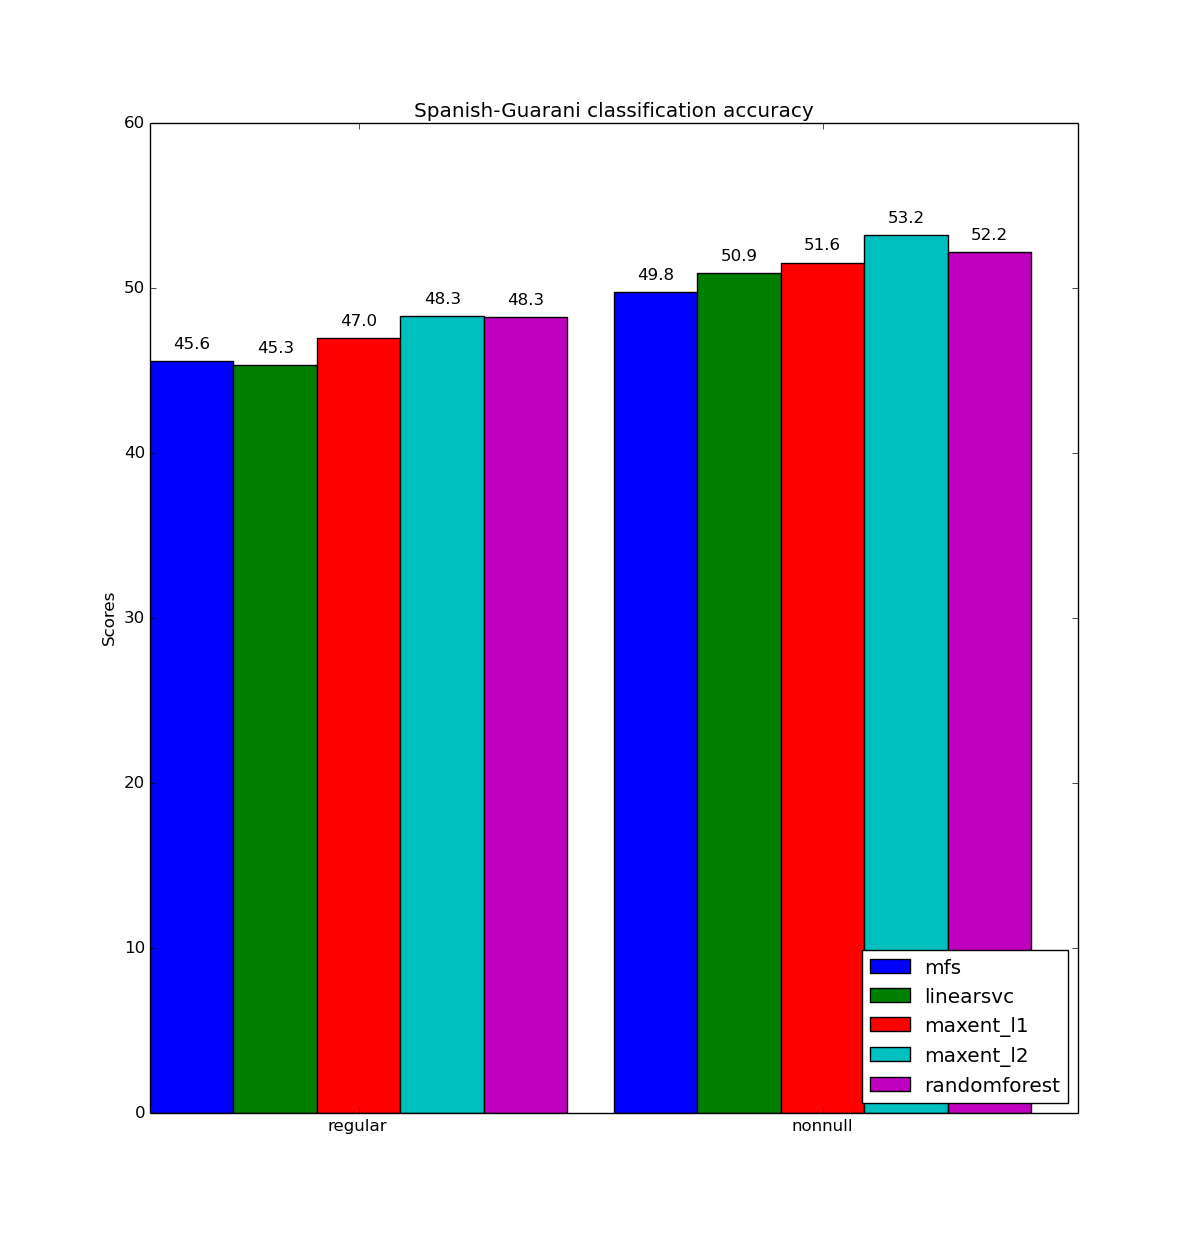
\includegraphics[width=\textwidth]{baseline-esgn-ch4.png}
  \caption{Baseline Chipa scores for Spanish-Guaraní, by classifier.}
  \label{fig:esgnresults:monolingual}
\end{figure}

\begin{figure}
  %% 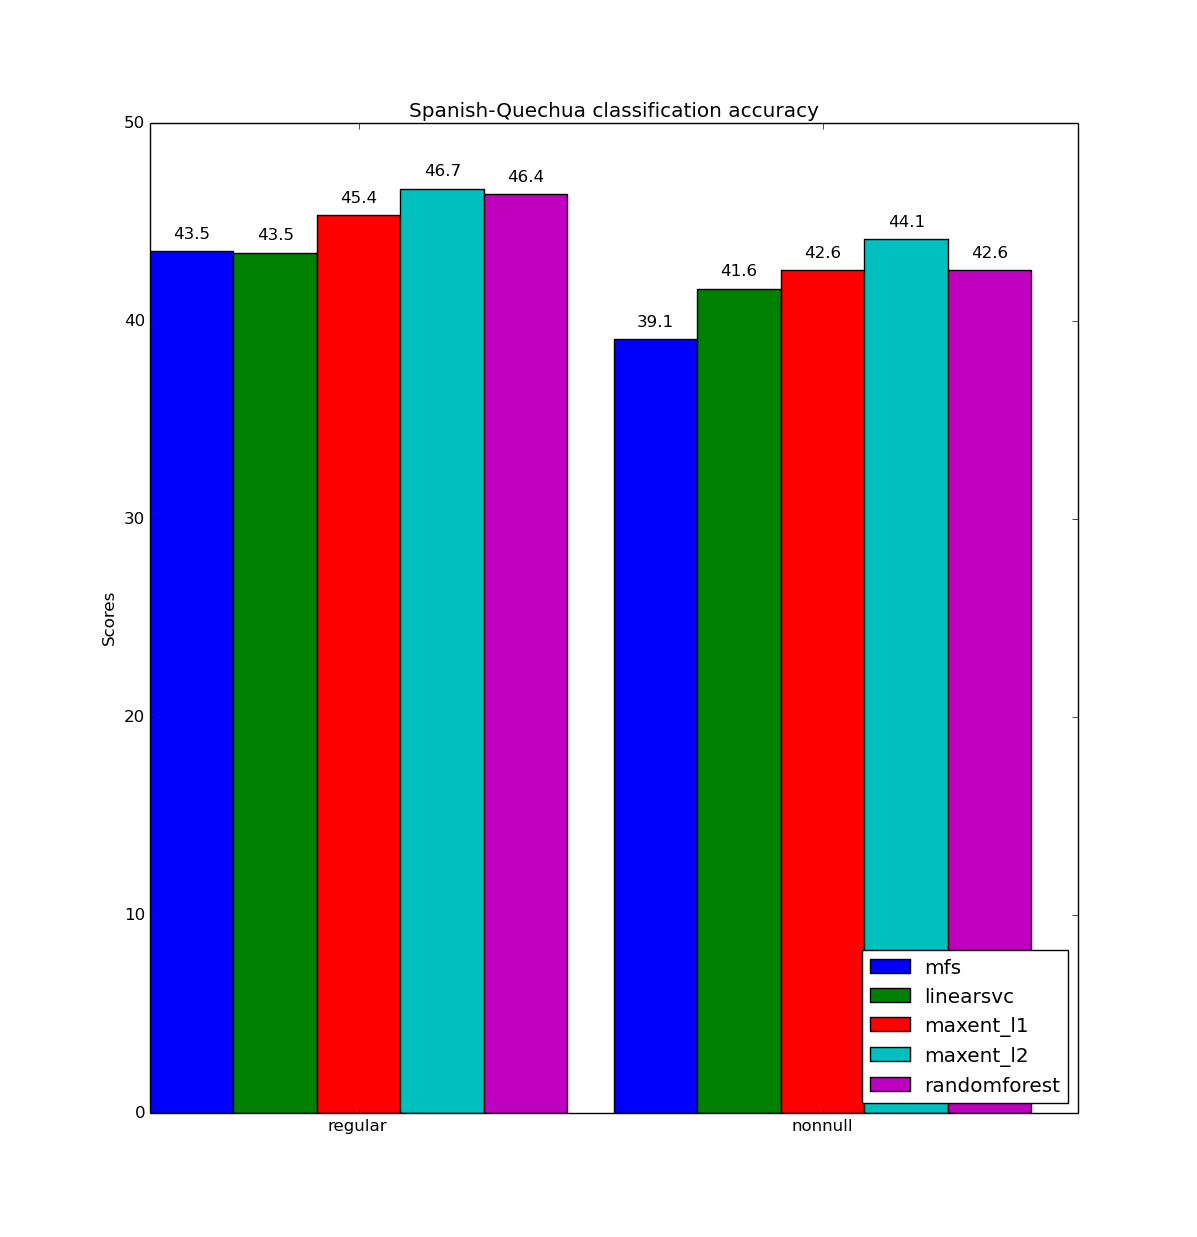
\includegraphics[width=\textwidth]{baseline-esqu-ch4.png}
  \caption{Baseline Chipa scores for Spanish-Quechua, by classifier.}
  \label{fig:esquresults:monolingual}
\end{figure}


\section{Discussion}
In this chapter, we have shown a number of different approaches that we can
leverage resources for our source language, including three different ways of
learning from unannotated source-language text and making use of existing
source-language syntactic analysis tools.

Using each of these different tools, we were able to overcome the relatively
strong most-frequent sense baseline, and with many of them, we were able to
improve slightly on the default feature set, described in the previous chapter.
All of these approaches make more abstract representations of the source text
available to our classifiers, whether these representations were learned from
the available text, or encapsulate some kind of syntactic knowledge about the
language. We found, in general, that representing the text closely surrounding
the focus word was more effective than attempting to represent the entire
source-language sentence at once.

In the next chapter, we will leverage another one of our important resources
that we have available for a resource-rich language like Spanish: bitext with
other language pairs.
